\section{Evaluation}

\begin{frame}{Evaluation}
    \begin{itemize}
        \item Accelerometer-based gesture detection inspired by \textit{uWave} \cite{liu2009uwave}

        \item 14 records of three-dimensional acceleration time series by 14 different experimentees

        \item Recorded via a Wii Remote\texttrademark~Plus Wii U is a trademark of Nintendo. controller
        \begin{center}
            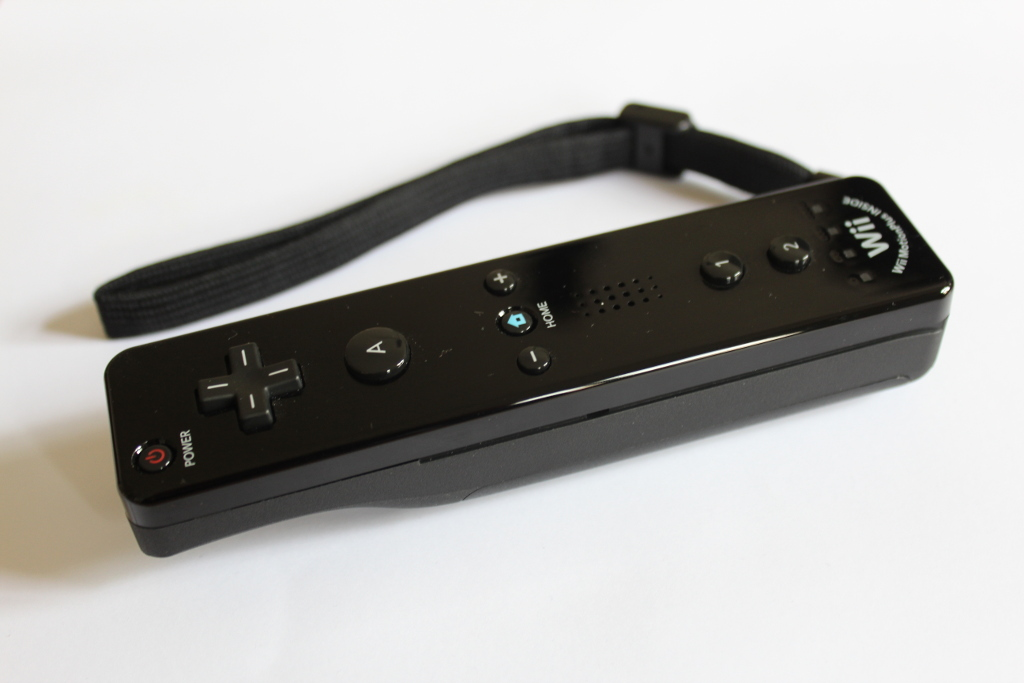
\includegraphics[width=0.5\textwidth]{wii-remote-plus-controller.JPG}
        \end{center}
    \end{itemize}
\end{frame}

\begin{frame}{Evaluation}{Data Recording Instructions}
    \begin{center}
        \resizebox {\textwidth} {!} {
            \begin{tabular}{ccccc}
                \frame{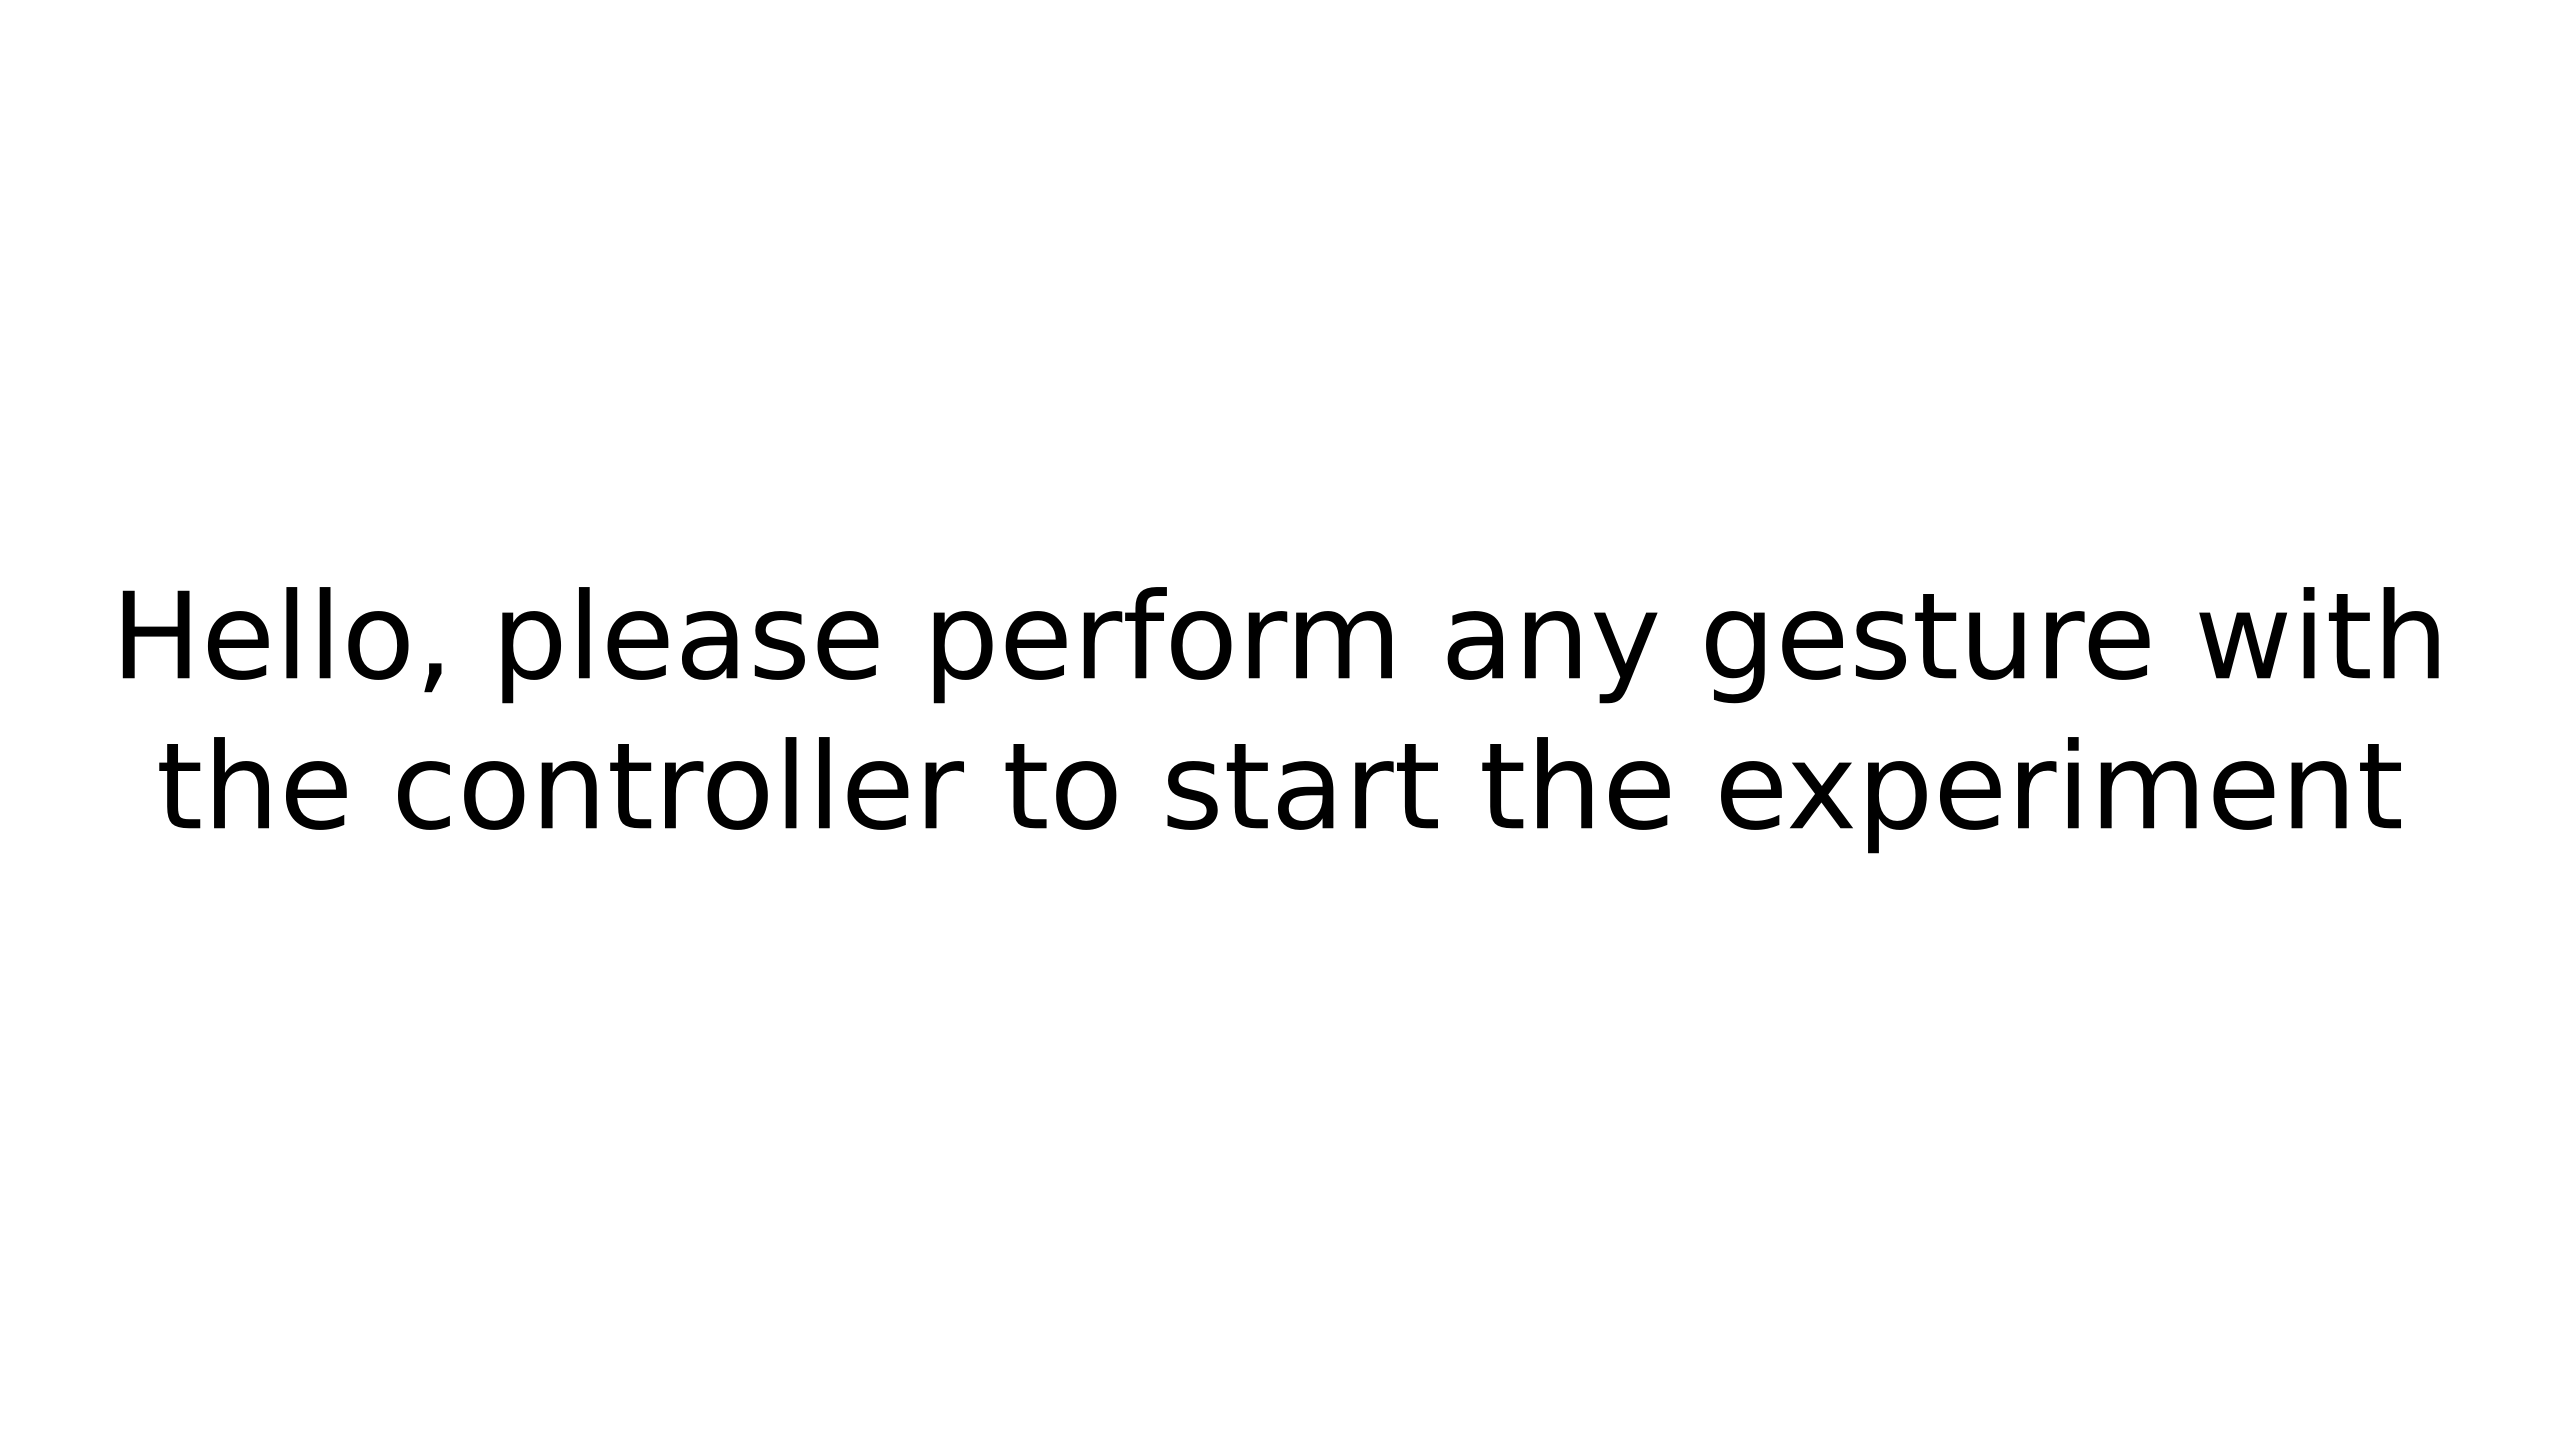
\includegraphics[width=0.25\textwidth]{1.png}} &
                \frame{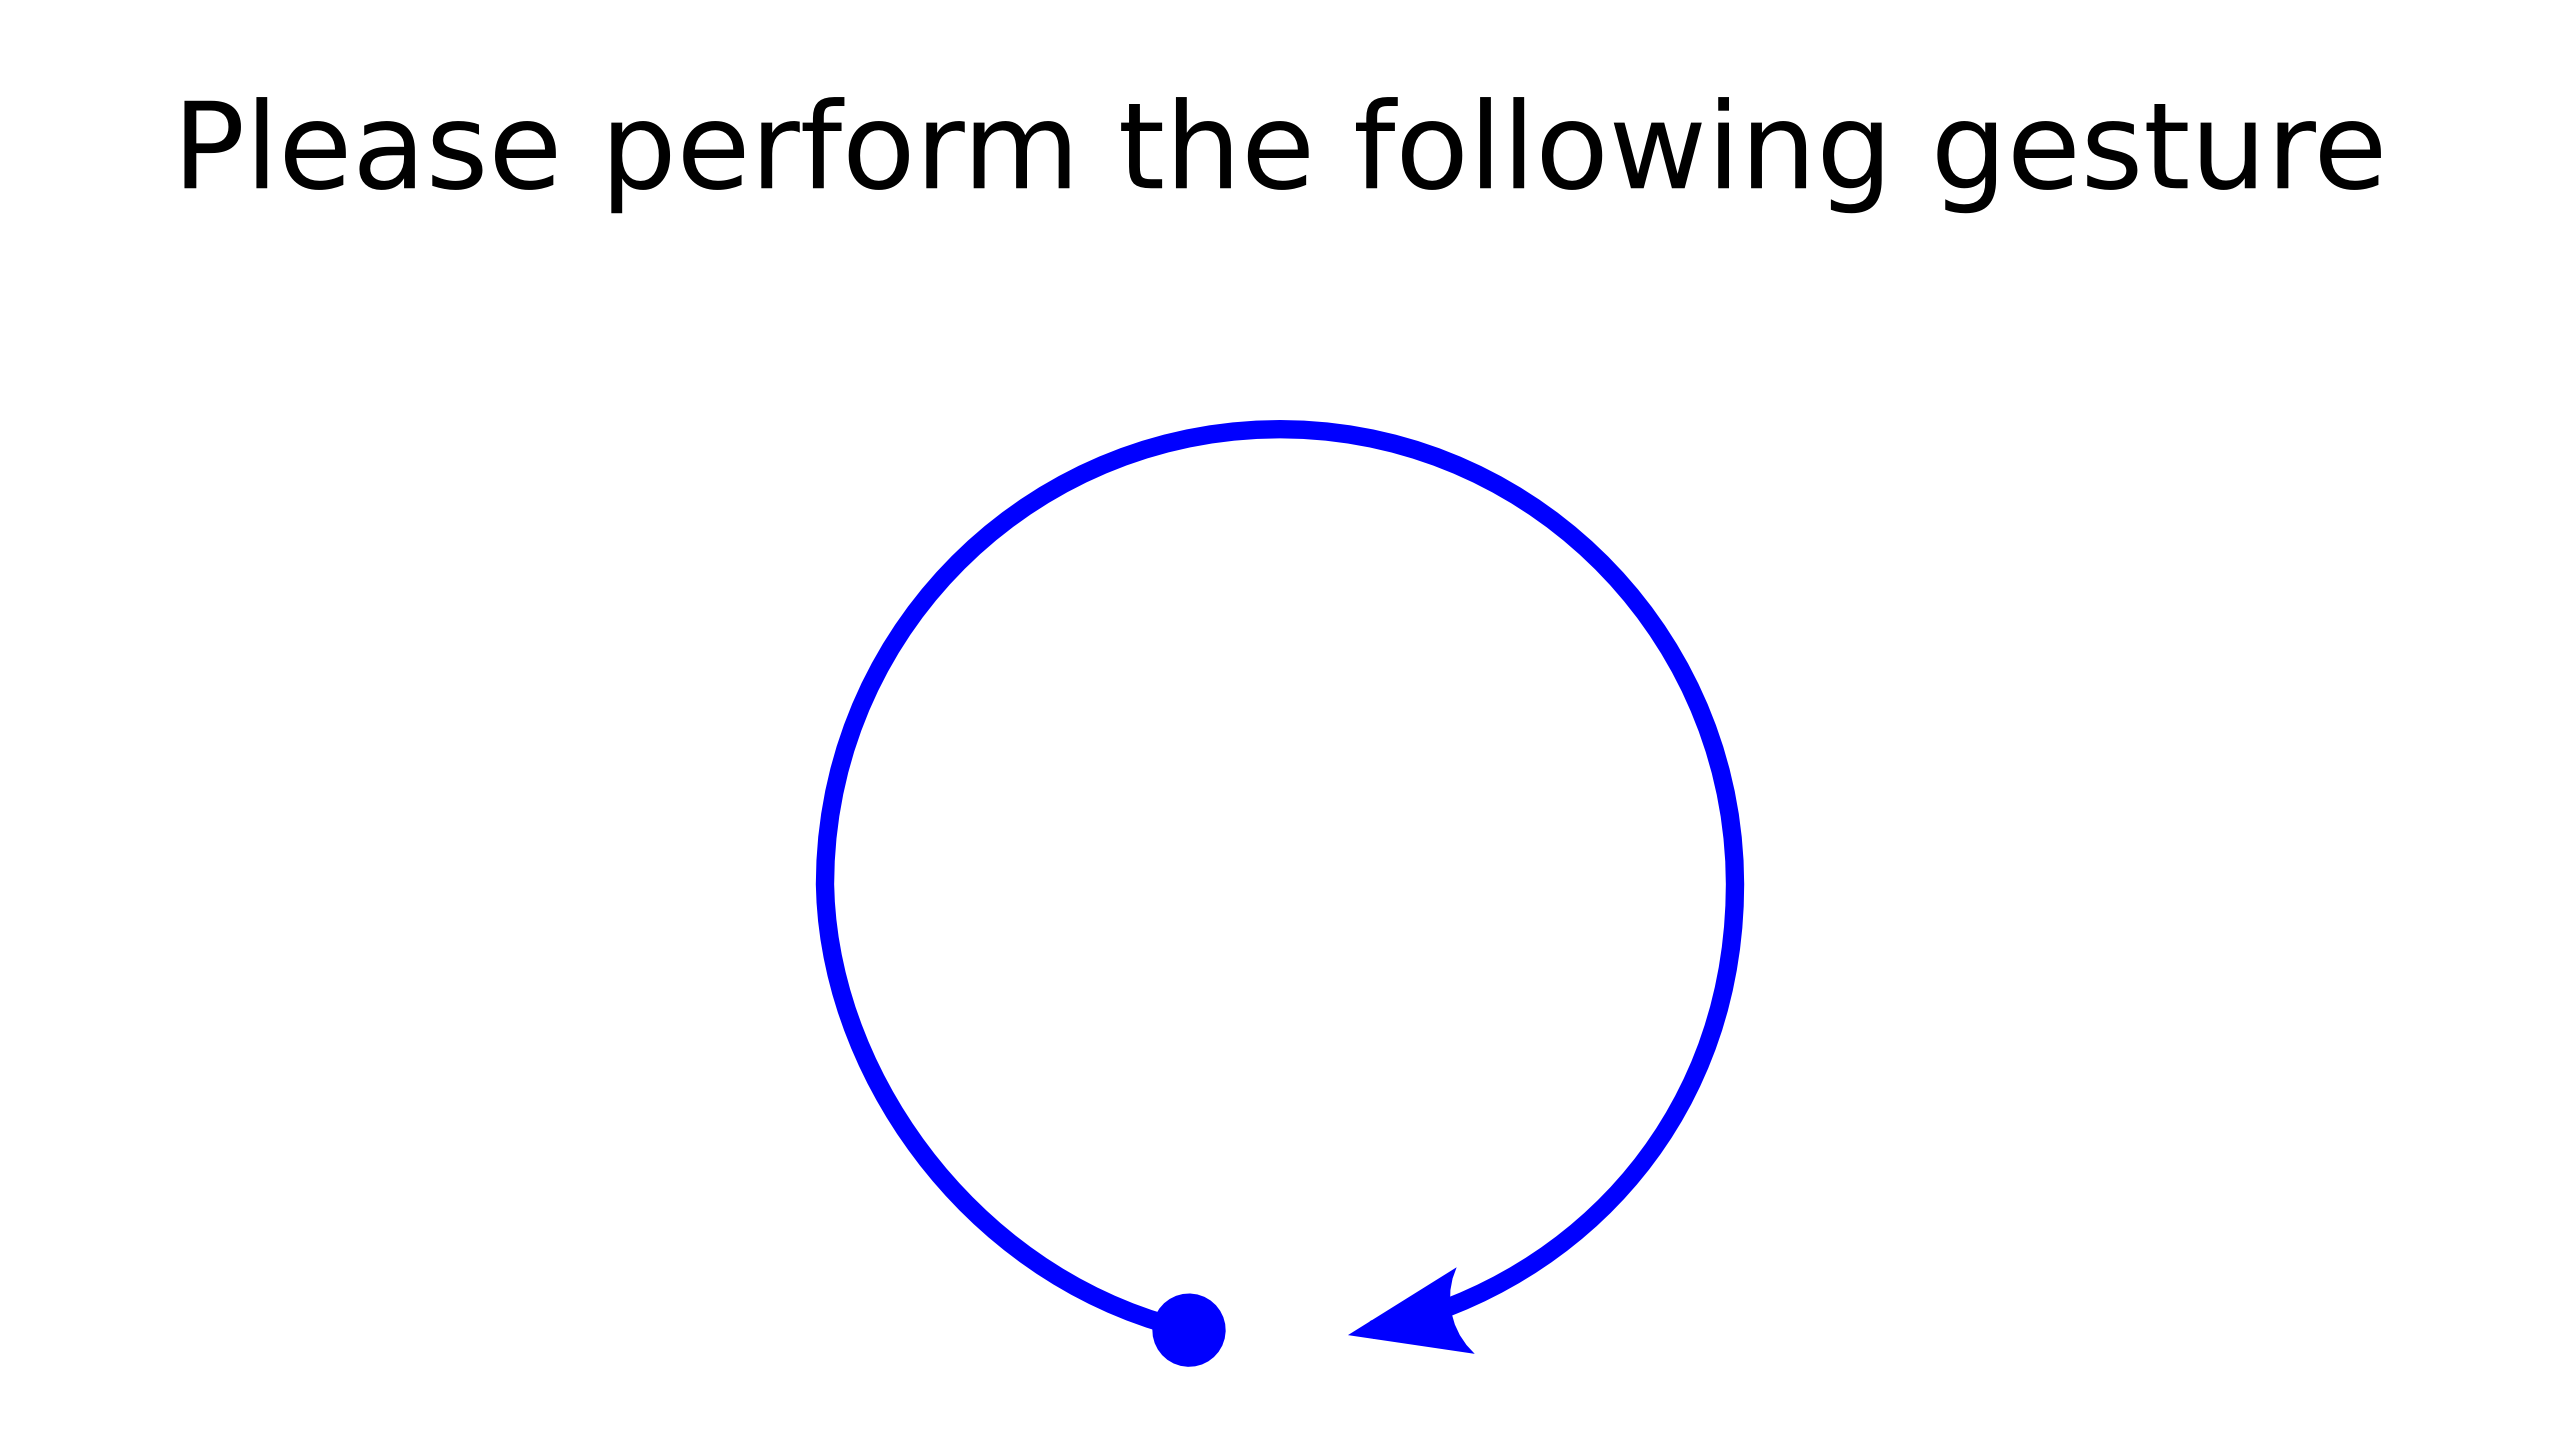
\includegraphics[width=0.25\textwidth]{2.png}} &
                \frame{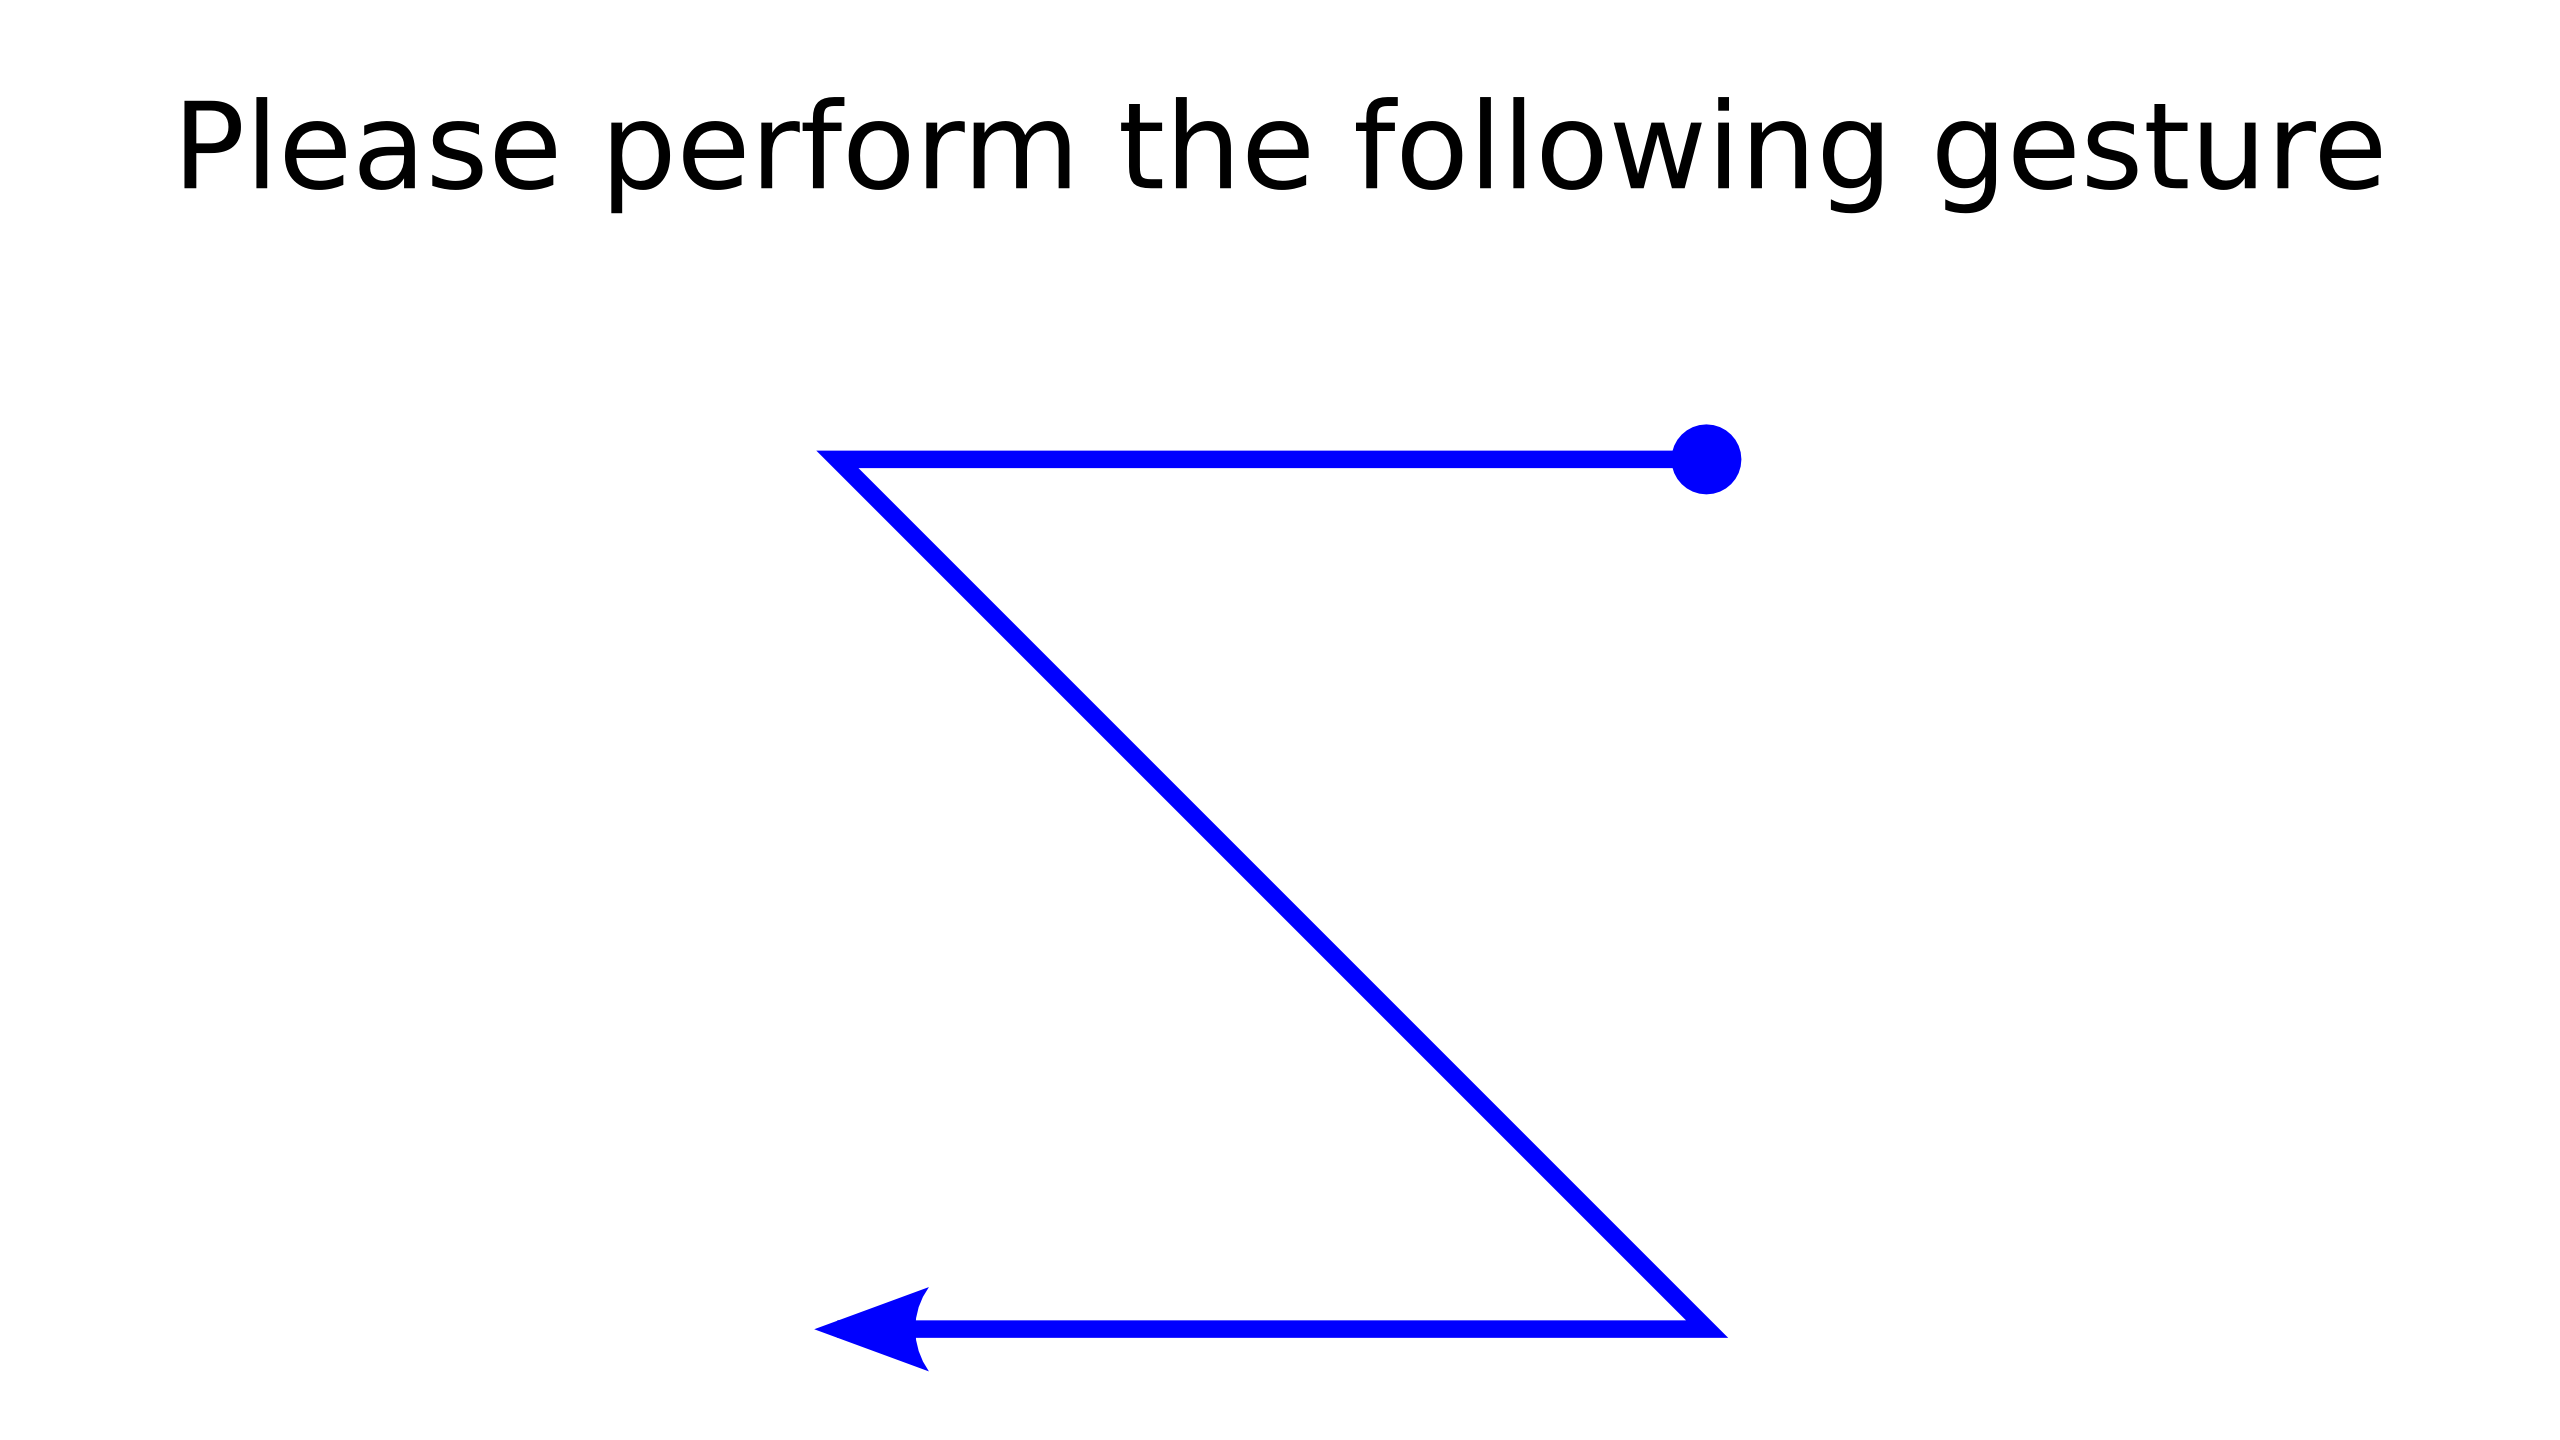
\includegraphics[width=0.25\textwidth]{3.png}} &
                \frame{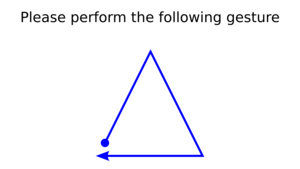
\includegraphics[width=0.25\textwidth]{4.png}} &
                \frame{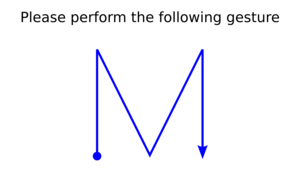
\includegraphics[width=0.25\textwidth]{5.png}} \\
                \frame{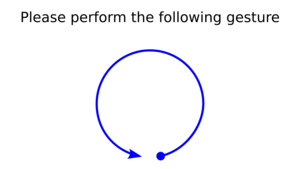
\includegraphics[width=0.25\textwidth]{6.png}} &
                \frame{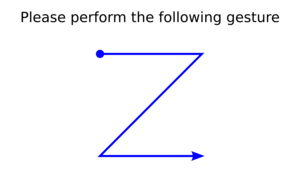
\includegraphics[width=0.25\textwidth]{7.png}} &
                \frame{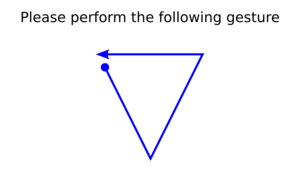
\includegraphics[width=0.25\textwidth]{8.png}} &
                \frame{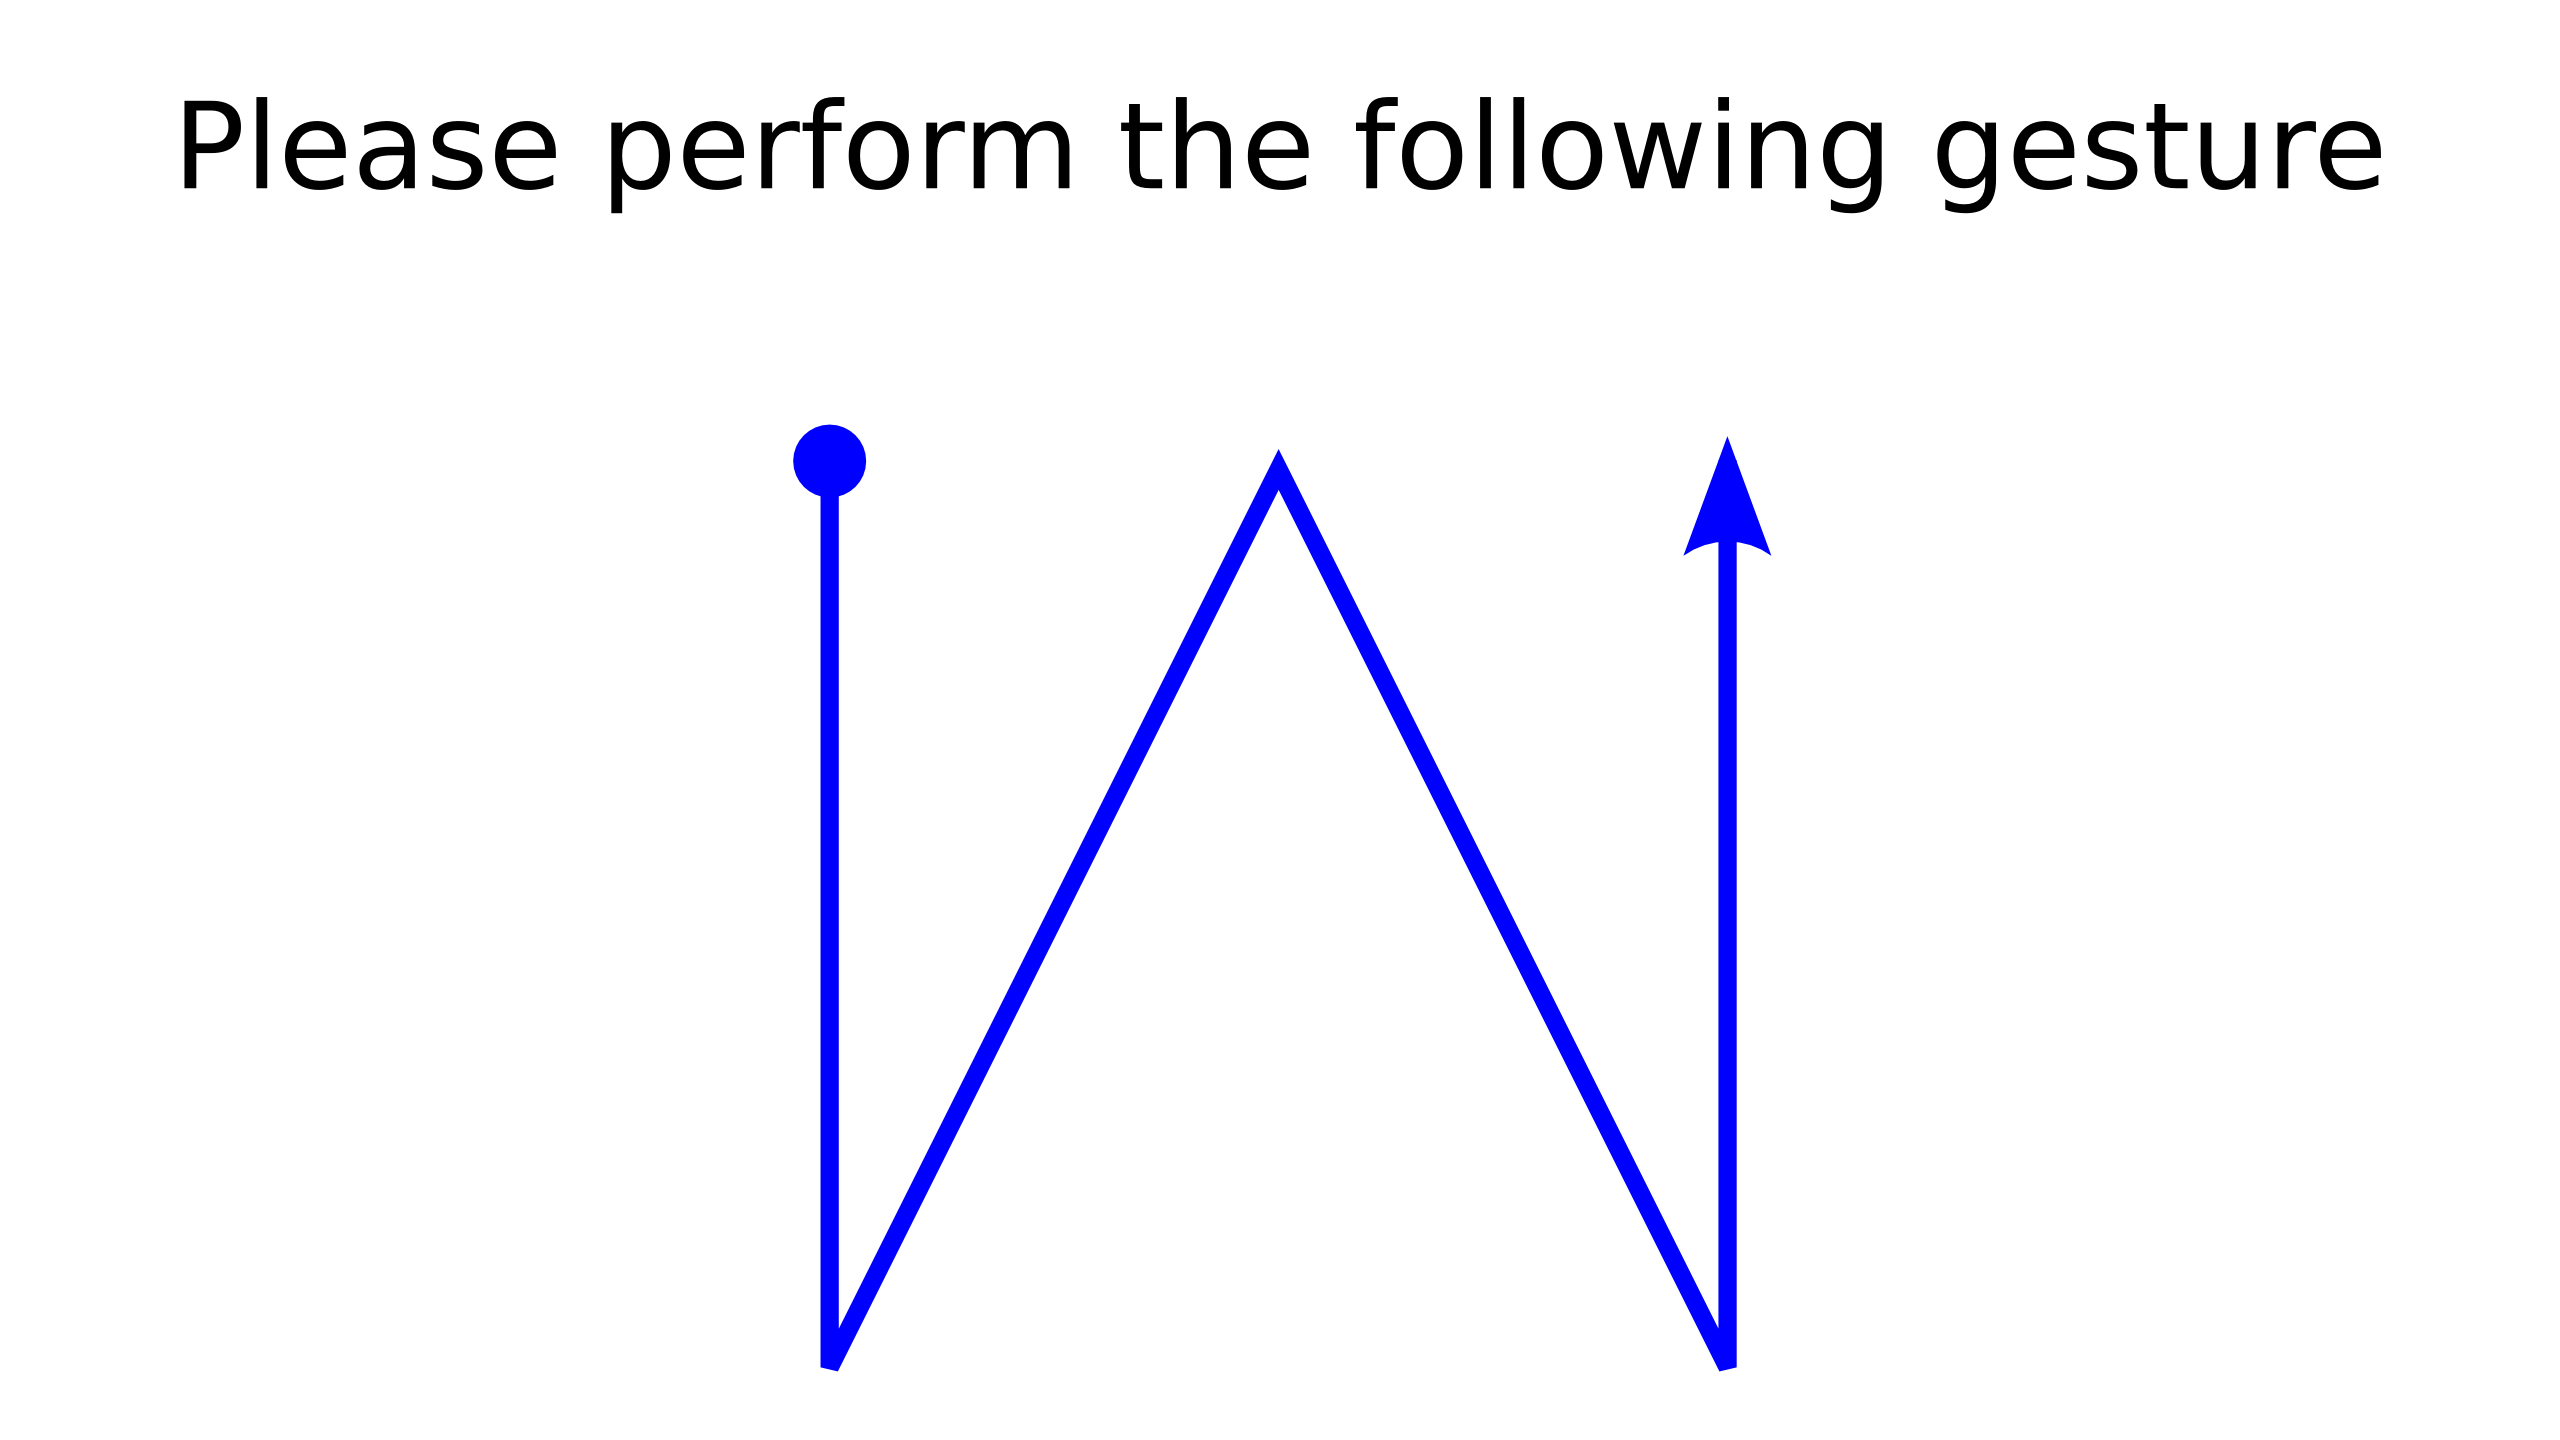
\includegraphics[width=0.25\textwidth]{9.png}} &
                \frame{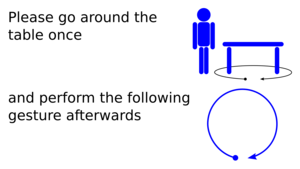
\includegraphics[width=0.25\textwidth]{10.png}} \\
                \frame{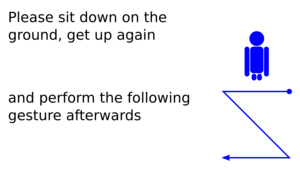
\includegraphics[width=0.25\textwidth]{11.png}} &
                \frame{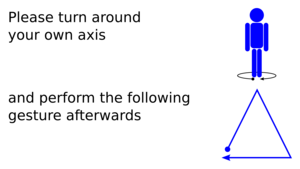
\includegraphics[width=0.25\textwidth]{12.png}} &
                \frame{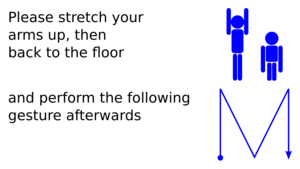
\includegraphics[width=0.25\textwidth]{13.png}} &
                \frame{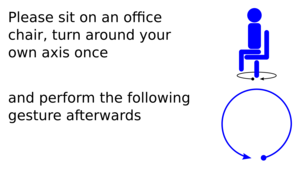
\includegraphics[width=0.25\textwidth]{14.png}} &
                \frame{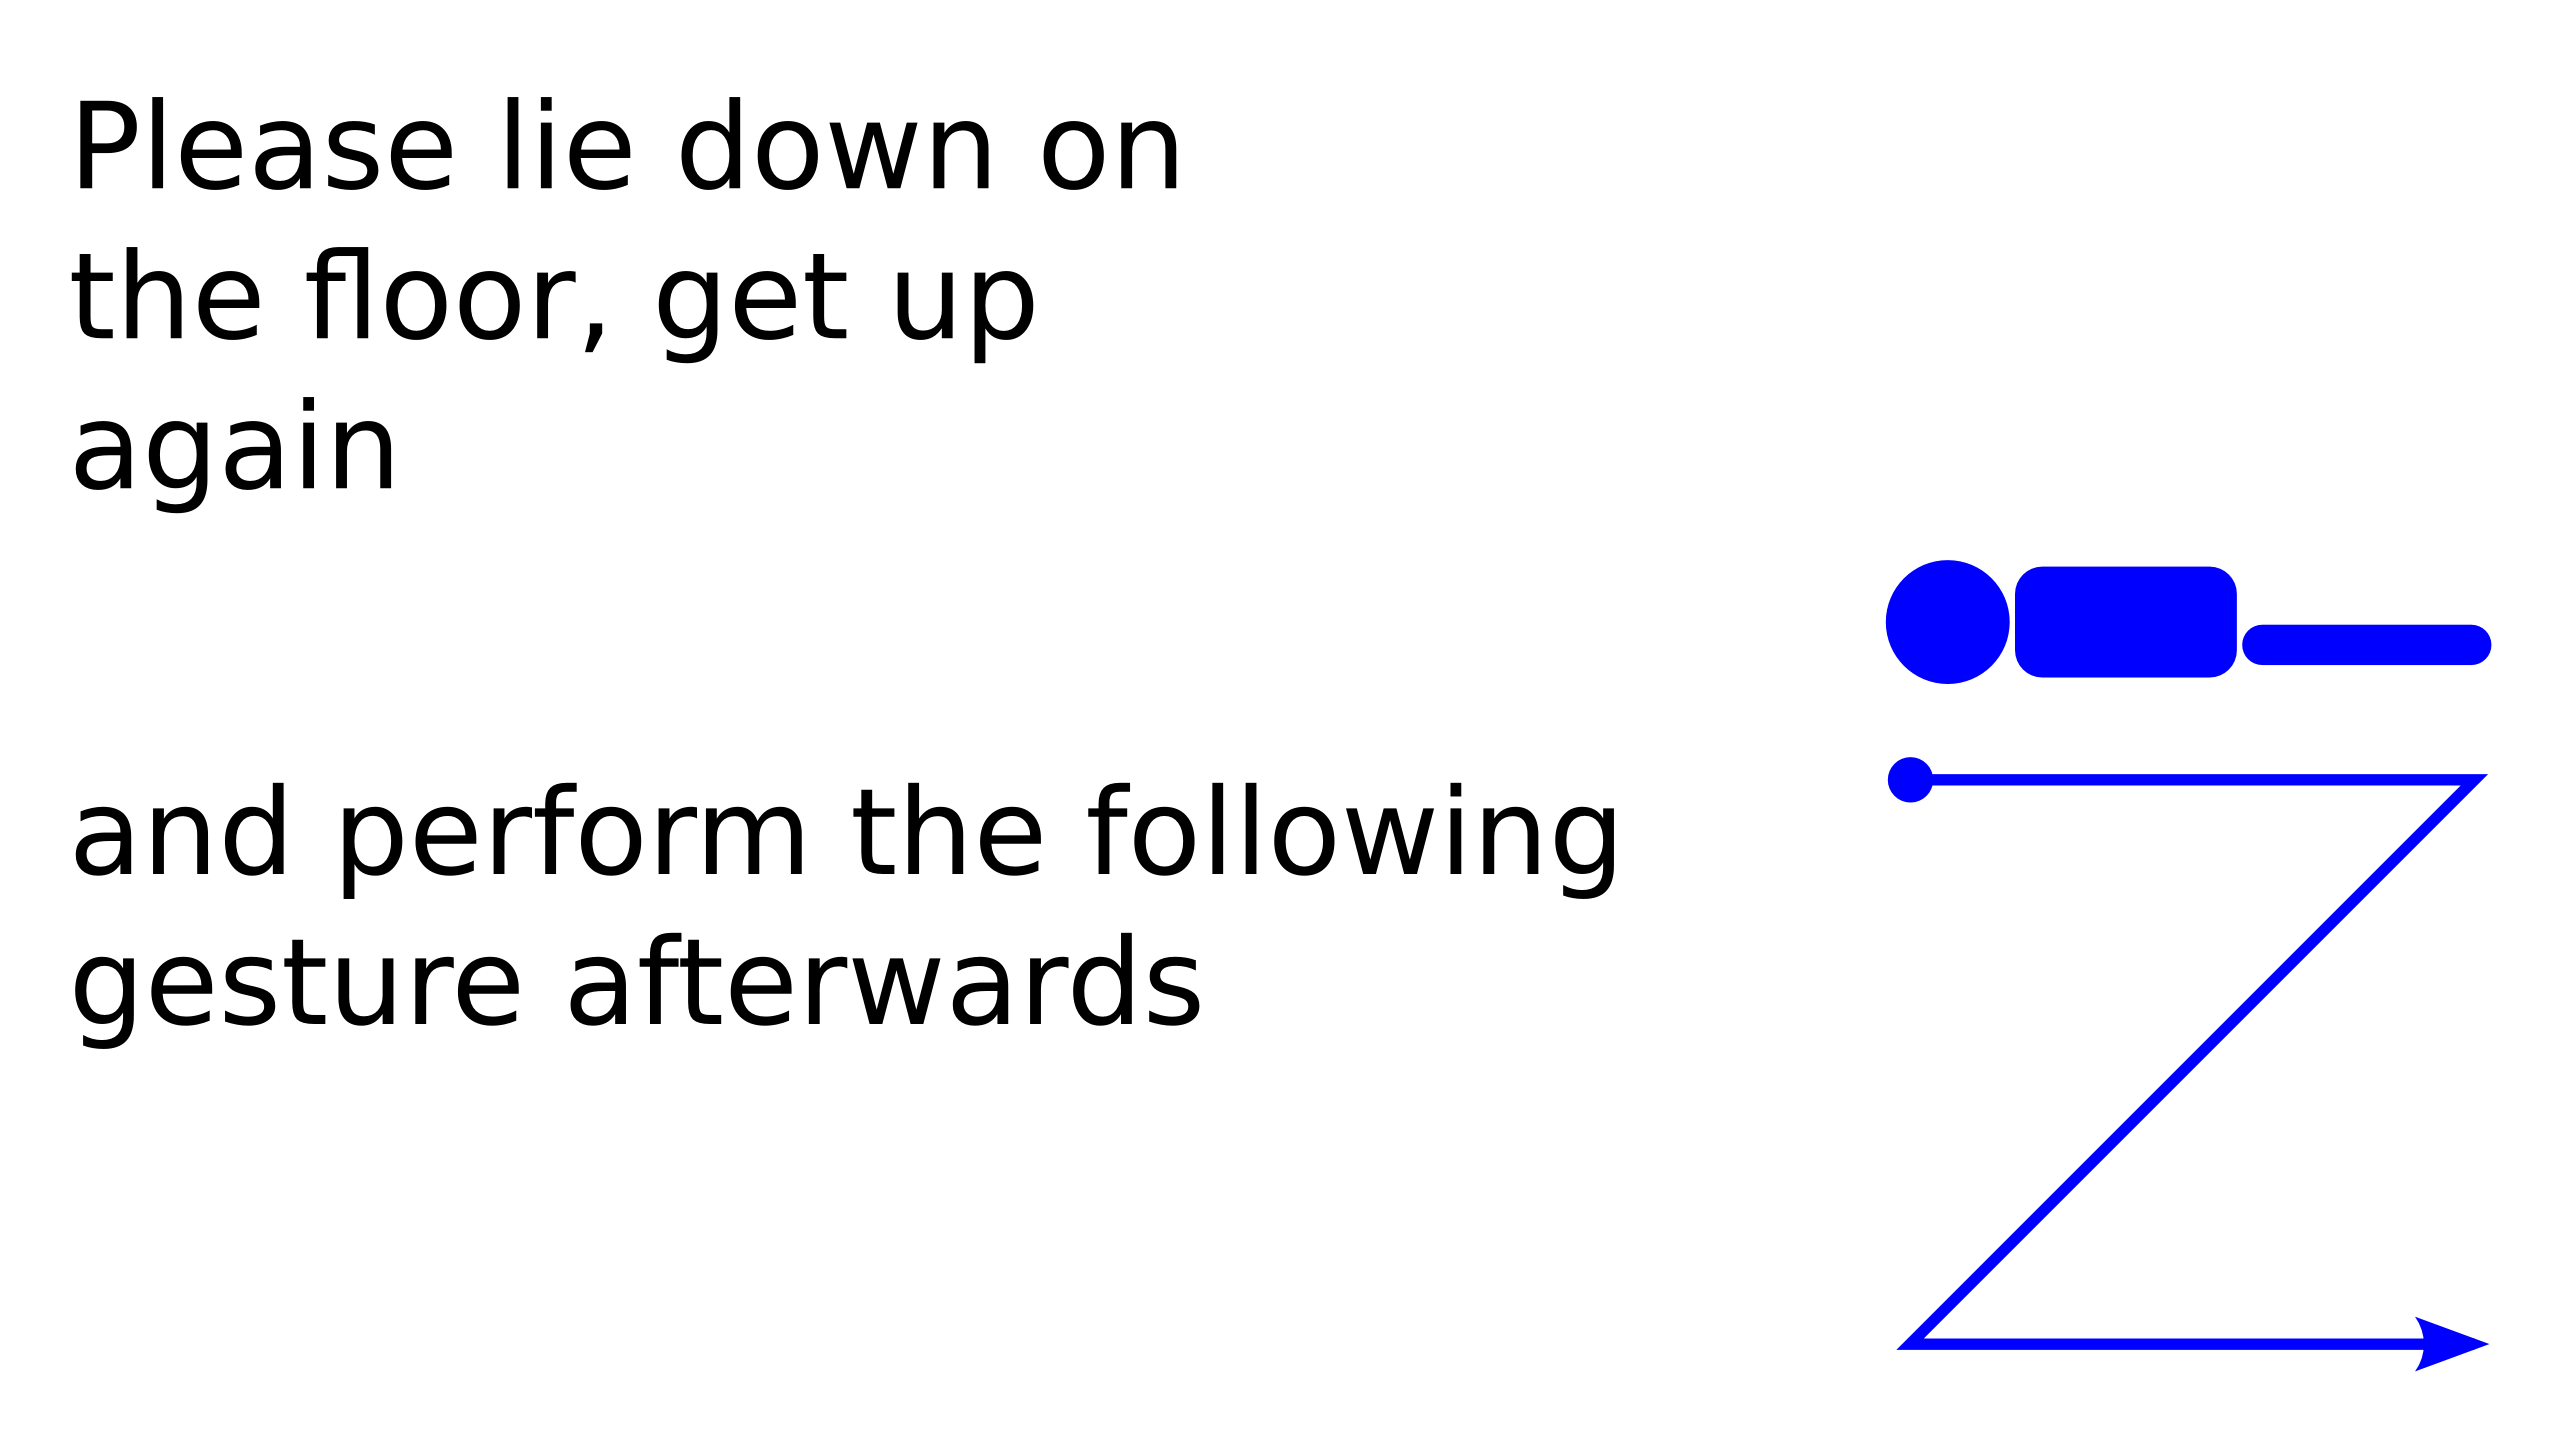
\includegraphics[width=0.25\textwidth]{15.png}} \\
                \frame{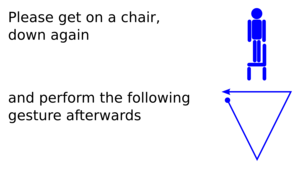
\includegraphics[width=0.25\textwidth]{16.png}} &
                \frame{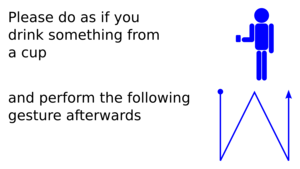
\includegraphics[width=0.25\textwidth]{17.png}} &
                \frame{
\includegraphics[width=0.25\textwidth]{18.png}} &
                \frame{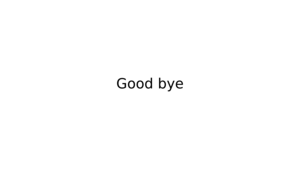
\includegraphics[width=0.25\textwidth]{19.png}} \\
            \end{tabular}
        }
    \end{center}
\end{frame}

\begin{frame}{Evaluation}{Recording Example}
    \resizebox {\textwidth} {!} {
        \begin{tikzpicture}
            \begin{axis}[
                xmin=0,
                xmax=3176,
                ymin=-16,
                ymax=16,
                width=10*\axisdefaultwidth,
                height=\axisdefaultheight,
                xticklabels={,,},
                yticklabels={,,}]
                \addplot[blue, mark=none, opacity=0.4] table[x=t, y=x] {../data/fig/record1/timeseries.dat};
                \addplot[red, mark=none, opacity=0.4] table[x=t, y=y] {../data/fig/record1/timeseries.dat};
                \addplot[green, mark=none, opacity=0.4] table[x=t, y=z] {../data/fig/record1/timeseries.dat};
                \addplot+[fill, opacity=0.5, blue, mark=none] coordinates {(38, -16) (89, -16) (89, 16) (38, 16)} --cycle;
                \addplot+[fill, opacity=0.5, blue, mark=none] coordinates {(123, -16) (177, -16) (177, 16) (123, 16)} --cycle;
                \addplot+[fill, opacity=0.5, blue, mark=none] coordinates {(201, -16) (256, -16) (256, 16) (201, 16)} --cycle;
                \addplot+[fill, opacity=0.5, blue, mark=none] coordinates {(282, -16) (355, -16) (355, 16) (282, 16)} --cycle;
                \addplot+[fill, opacity=0.5, blue, mark=none] coordinates {(388, -16) (439, -16) (439, 16) (388, 16)} --cycle;
                \addplot+[fill, opacity=0.5, blue, mark=none] coordinates {(473, -16) (530, -16) (530, 16) (473, 16)} --cycle;
                \addplot+[fill, opacity=0.5, blue, mark=none] coordinates {(568, -16) (624, -16) (624, 16) (568, 16)} --cycle;
                \addplot+[fill, opacity=0.5, blue, mark=none] coordinates {(672, -16) (749, -16) (749, 16) (672, 16)} --cycle;
                \addplot+[fill, opacity=0.5, blue, mark=none] coordinates {(1057, -16) (1106, -16) (1106, 16) (1057, 16)} --cycle;
                \addplot+[fill, opacity=0.5, blue, mark=none] coordinates {(1258, -16) (1313, -16) (1313, 16) (1258, 16)} --cycle;
                \addplot+[fill, opacity=0.5, blue, mark=none] coordinates {(1472, -16) (1527, -16) (1527, 16) (1472, 16)} --cycle;
                \addplot+[fill, opacity=0.5, blue, mark=none] coordinates {(1690, -16) (1772, -16) (1772, 16) (1690, 16)} --cycle;
                \addplot+[fill, opacity=0.5, blue, mark=none] coordinates {(2066, -16) (2116, -16) (2116, 16) (2066, 16)} --cycle;
                \addplot+[fill, opacity=0.5, blue, mark=none] coordinates {(2439, -16) (2497, -16) (2497, 16) (2439, 16)} --cycle;
                \addplot+[fill, opacity=0.5, blue, mark=none] coordinates {(2840, -16) (2895, -16) (2895, 16) (2840, 16)} --cycle;
                \addplot+[fill, opacity=0.5, blue, mark=none] coordinates {(3061, -16) (3137, -16) (3137, 16) (3061, 16)} --cycle;
            \end{axis}
        \end{tikzpicture}
    }
\end{frame}

\begin{frame}{Evaluation}{Data Preparation}
    \begin{itemize}
        \item \textit{Resampling}: data was resampled by means of the moving average technique, using a window size of 50 ms and step size of 30 ms
        \item \textit{Quantization}: converted into time series with integer values between -16 and 16, such as suggested in related work \cite{liu2009uwave}\\
        \begin{center}
            \tiny
            \begin{tabular}{cc}
                \hline
                \textbf{Acceleration data ($a$) in $\frac{dm}{s^2}$} & \textbf{Converted value}\\
                \hline
                $a > 200$ & 16\\
                $100 < a < 200$ & 11 to 15 (five levels linearly)\\
                $0 < a < 100$ & 1 to 10 (ten levels linearly)\\
                $a = 0$ & 0\\
                $-100 < a < 0$ & -1 to - 10 (ten levels linearly)\\
                $-200 < a < -100$ & -11 to - 15 (five levels linearly)\\
                $a < -200$ & -16\\
                \hline
            \end{tabular}
        \end{center}
    \end{itemize}
\end{frame}

\begin{frame}{Evaluation}{Data Preparation Example}
    \begin{center}
        \resizebox {\textwidth} {!} {
            \begin{tabular}{ccc}
                \resizebox {!} {\height} {
                    \begin{tikzpicture}
                        \begin{axis}[
                            xmin=1,
                            xmax=295,
                            xlabel=time,
                            ylabel=acceleration in $\frac{dm}{s^2}$]
                            \addplot[blue, ultra thick, mark=none] table[x=t, y=x] {../data/fig/quantization/raw.dat};
                            \addplot[red, ultra thick, mark=none] table[x=t, y=y] {../data/fig/quantization/raw.dat};
                            \addplot[green, ultra thick, mark=none] table[x=t, y=z] {../data/fig/quantization/raw.dat};
                        \end{axis}
                    \end{tikzpicture}
                } &
                \resizebox {!} {\height} {
                    \begin{tikzpicture}
                        \pgfplotsset{every axis legend/.append style={
                    		at={(0.5,1.03)},
                    		anchor=south}}
                        \begin{axis}[
                            xmin=1,
                            xmax=52,
                            xlabel=time,
                            ylabel=acceleration in $\frac{dm}{s^2}$,
                            legend columns=4]
                            \addplot[blue, ultra thick, mark=none] table[x=t, y=x] {../data/fig/quantization/compressed.dat};
                            \addlegendentry{x-axis}
                            \addplot[red, ultra thick, mark=none] table[x=t, y=y] {../data/fig/quantization/compressed.dat};
                            \addlegendentry{y-axis}
                            \addplot[green, ultra thick, mark=none] table[x=t, y=z] {../data/fig/quantization/compressed.dat};
                            \addlegendentry{z-axis}
                        \end{axis}
                    \end{tikzpicture}
                } &
                \resizebox {!} {\height} {
                    \begin{tikzpicture}
                        \begin{axis}[
                            xmin=1,
                            xmax=52,
                            xlabel=time,
                            ylabel=converted acceleration]
                            \addplot[blue, ultra thick, mark=none] table[x=t, y=x] {../data/fig/quantization/converted.dat};
                            \addplot[red, ultra thick, mark=none] table[x=t, y=y] {../data/fig/quantization/converted.dat};
                            \addplot[green, ultra thick, mark=none] table[x=t, y=z] {../data/fig/quantization/converted.dat};
                        \end{axis}
                    \end{tikzpicture}
                }
            \end{tabular}
        }
    \end{center}
\end{frame}

\begin{frame}{Experiment}{Model parameters}
    \begin{itemize}
        \item \textit{window size}: determines the number of most recent measurements
            \begin{itemize}
                \item min
                \item max
                \item avg
                \item mid
            \end{itemize}
        \item \textit{step size}: defines the gap between consecutive time series windows
            \begin{itemize}
                \item tenth of the window size
            \end{itemize}
        \item \textit{normalization}: normalization prior to pair-wise comparing sliding windows and training gestures
            \begin{itemize}
                \item $\eta$ normalization
                \item $z$ normalization
                \item no normalization
            \end{itemize}
    \end{itemize}
\end{frame}

\begin{frame}{Experiment}{Model Parameters}
    \begin{itemize}
        \item \textit{Sakoe-Chiba band sizes}:
            \begin{itemize}
                \item 34 different between 1 \% to 100 \%
            \end{itemize}
        \item \textit{threshold}: defines the time series distance at which a sliding window and a training gesture are considered to belong to the same class
            \begin{itemize}
                \item HMinD
                \item HAvgD
                \item HMidD
            \end{itemize}
        \item \textit{filter criterion}:
            \begin{itemize}
                \item VAR
                \item LNCE
                \item no filter
            \end{itemize}
    \end{itemize}
\end{frame}

\begin{frame}{Experiment}{Example Result}
    \resizebox {\textwidth} {!} {
        \begin{tikzpicture}
            \begin{axis}[
                xmin=0,
                xmax=2426,
                ymin=-16,
                ymax=16,
                width=10*\axisdefaultwidth,
                height=\axisdefaultheight,
                xticklabels={,,},
                yticklabels={,,}]
                \addplot[blue, mark=none, opacity=0.4] table[x=t, y=x] {../data/fig/experimentee_result2/exp1.dat};
                \addplot[red, mark=none, opacity=0.4] table[x=t, y=y] {../data/fig/experimentee_result2/exp1.dat};
                \addplot[green, mark=none, opacity=0.4] table[x=t, y=z] {../data/fig/experimentee_result2/exp1.dat};
                \addplot+[fill, opacity=0.5, red, mark=none] coordinates {(294, -16) (307, -16) (307, 16) (294, 16)} --cycle;
                \addplot+[fill, opacity=0.5, green, mark=none] coordinates {(307, -16) (357, -16) (357, 16) (307, 16)} --cycle;
                \addplot+[fill, opacity=0.5, red, mark=none] coordinates {(357, -16) (359, -16) (359, 16) (357, 16)} --cycle;
                \addplot+[fill, opacity=0.5, red, mark=none] coordinates {(497, -16) (508, -16) (508, 16) (497, 16)} --cycle;
                \addplot+[fill, opacity=0.5, green, mark=none] coordinates {(508, -16) (562, -16) (562, 16) (508, 16)} --cycle;
                \addplot+[fill, opacity=0.5, blue, mark=none] coordinates {(562, -16) (564, -16) (564, 16) (562, 16)} --cycle;
                \addplot+[fill, opacity=0.5, red, mark=none] coordinates {(712, -16) (722, -16) (722, 16) (712, 16)} --cycle;
                \addplot+[fill, opacity=0.5, green, mark=none] coordinates {(722, -16) (777, -16) (777, 16) (722, 16)} --cycle;
                \addplot+[fill, opacity=0.5, blue, mark=none] coordinates {(777, -16) (778, -16) (778, 16) (777, 16)} --cycle;
                \addplot+[fill, opacity=0.5, blue, mark=none] coordinates {(940, -16) (945, -16) (945, 16) (940, 16)} --cycle;
                \addplot+[fill, opacity=0.5, green, mark=none] coordinates {(945, -16) (1010, -16) (1010, 16) (945, 16)} --cycle;
                \addplot+[fill, opacity=0.5, blue, mark=none] coordinates {(1010, -16) (1023, -16) (1023, 16) (1010, 16)} --cycle;
                \addplot+[fill, opacity=0.5, red, mark=none] coordinates {(1310, -16) (1316, -16) (1316, 16) (1310, 16)} --cycle;
                \addplot+[fill, opacity=0.5, green, mark=none] coordinates {(1316, -16) (1367, -16) (1367, 16) (1316, 16)} --cycle;
                \addplot+[fill, opacity=0.5, red, mark=none] coordinates {(1367, -16) (1375, -16) (1375, 16) (1367, 16)} --cycle;
                \addplot+[fill, opacity=0.5, red, mark=none] coordinates {(1681, -16) (1689, -16) (1689, 16) (1681, 16)} --cycle;
                \addplot+[fill, opacity=0.5, green, mark=none] coordinates {(1689, -16) (1746, -16) (1746, 16) (1689, 16)} --cycle;
                \addplot+[fill, opacity=0.5, blue, mark=none] coordinates {(1746, -16) (1748, -16) (1748, 16) (1746, 16)} --cycle;
                \addplot+[fill, opacity=0.5, red, mark=none] coordinates {(2082, -16) (2090, -16) (2090, 16) (2082, 16)} --cycle;
                \addplot+[fill, opacity=0.5, green, mark=none] coordinates {(2090, -16) (2146, -16) (2146, 16) (2090, 16)} --cycle;
                \addplot+[fill, opacity=0.5, red, mark=none] coordinates {(2146, -16) (2147, -16) (2147, 16) (2146, 16)} --cycle;
                \addplot+[fill, opacity=0.5, blue, mark=none] coordinates {(2311, -16) (2388, -16) (2388, 16) (2311, 16)} --cycle;
                \addplot+[fill, opacity=0.5, red, mark=none] coordinates {(2297, -16) (2362, -16) (2362, 16) (2297, 16)} --cycle;
            \end{axis}
        \end{tikzpicture}
    }
\end{frame}

\begin{frame}{Evaluation}{Simulations ranked by $F_{1}score_{\mu}$}
    \begin{center}
        \resizebox {0.5\textwidth} {!} {
            \begin{tikzpicture}[spy using outlines={circle, magnification=6, connect spies}]
                \begin{axis}[
                    xmin=0,
                    xmax=1,
                    ymin=0,
                    ymax=1,
                    width=\axisdefaultwidth,
                    height=\axisdefaultwidth,
                    xlabel=$Precision_{\mu}$,
                    ylabel=$Recall_{\mu}$,
                    samples=100,
                    colorbar horizontal,
                    colormap/viridis high res,
                    title=$F_{1}score_{\mu}$]
                    \addplot[only marks, scatter, scatter src=explicit, mark size=1] table[x=x,y=y,meta=fscore] {../data/fig/result2/result.dat};
                    \addplot[gray, domain=0.051:1] {(0.1 * x) / (2 * x - 0.1)};
                    \addplot[gray, domain=0.11:1] {(0.2 * x) / (2 * x - 0.2)};
                    \addplot[gray, domain=0.16:1] {(0.3 * x) / (2 * x - 0.3)};
                    \addplot[gray, domain=0.21:1] {(0.4 * x) / (2 * x - 0.4)};
                    \addplot[gray, domain=0.26:1] {(0.5 * x) / (2 * x - 0.5)};
                    \addplot[gray, domain=0.31:1] {(0.6 * x) / (2 * x - 0.6)};
                    \addplot[gray, domain=0.36:1] {(0.7 * x) / (2 * x - 0.7)};
                    \addplot[gray, domain=0.41:1] {(0.8 * x) / (2 * x - 0.8)};
                    \addplot[gray, domain=0.46:1] {(0.9 * x) / (2 * x - 0.9)};
                    \coordinate (spypoint) at (axis cs:0.8413867433,0.6578651685);
                    \coordinate (magnifyglass) at (axis cs:0.2,0.8);
                \end{axis}
                \spy [size=2cm] on (spypoint)
                    in node[fill=white] at (magnifyglass);
            \end{tikzpicture}
        }
    \end{center}
\end{frame}
